\documentclass{tufte-book}\usepackage{knitr}
\hypersetup{colorlinks}% uncomment this line if you prefer colored hyperlinks (e.g., for onscreen viewing)
%%
% Book metadata
\title{Quantitative Ecotoxicology}
\subtitle{with R!}
\author{Eduard Sz\"ocs}
%\publisher{Publisher of This Book}

%%
% For nicely typeset tabular material
\usepackage{booktabs}

%%
% For graphics / images
\usepackage{graphicx}
\setkeys{Gin}{width=\linewidth,totalheight=\textheight,keepaspectratio}
\graphicspath{{graphics/}}

% The fancyvrb package lets us customize the formatting of verbatim
% environments.  We use a slightly smaller font.
\usepackage{fancyvrb}
\fvset{fontsize=\normalsize}

%%
% Prints argument within hanging parentheses (i.e., parentheses that take
% up no horizontal space).  Useful in tabular environments.
\newcommand{\hangp}[1]{\makebox[0pt][r]{(}#1\makebox[0pt][l]{)}}

%%
% Prints an asterisk that takes up no horizontal space.
% Useful in tabular environments.
\newcommand{\hangstar}{\makebox[0pt][l]{*}}

%%
% Prints a trailing space in a smart way.
\usepackage{xspace}

%%
% Some shortcuts for Tufte's book titles.  The lowercase commands will
% produce the initials of the book title in italics.  The all-caps commands
% will print out the full title of the book in italics.
\newcommand{\vdqi}{\textit{VDQI}\xspace}
\newcommand{\ei}{\textit{EI}\xspace}
\newcommand{\ve}{\textit{VE}\xspace}
\newcommand{\be}{\textit{BE}\xspace}
\newcommand{\VDQI}{\textit{The Visual Display of Quantitative Information}\xspace}
\newcommand{\EI}{\textit{Envisioning Information}\xspace}
\newcommand{\VE}{\textit{Visual Explanations}\xspace}
\newcommand{\BE}{\textit{Beautiful Evidence}\xspace}

\newcommand{\TL}{Tufte-\LaTeX\xspace}

% Prints the month name (e.g., January) and the year (e.g., 2008)
\newcommand{\monthyear}{%
  \ifcase\month\or January\or February\or March\or April\or May\or June\or
  July\or August\or September\or October\or November\or
  December\fi\space\number\year
}


% Prints an epigraph and speaker in sans serif, all-caps type.
\newcommand{\openepigraph}[2]{%
  %\sffamily\fontsize{14}{16}\selectfont
  \begin{fullwidth}
  \sffamily\large
  \begin{doublespace}
  \noindent\allcaps{#1}\\% epigraph
  \noindent\allcaps{#2}% author
  \end{doublespace}
  \end{fullwidth}
}

% Inserts a blank page
\newcommand{\blankpage}{\newpage\hbox{}\thispagestyle{empty}\newpage}

\usepackage{units}

% Typesets the font size, leading, and measure in the form of 10/12x26 pc.
\newcommand{\measure}[3]{#1/#2$\times$\unit[#3]{pc}}

% Macros for typesetting the documentation
\newcommand{\hlred}[1]{\textcolor{Maroon}{#1}}% prints in red
\newcommand{\hangleft}[1]{\makebox[0pt][r]{#1}}
\newcommand{\hairsp}{\hspace{1pt}}% hair space
\newcommand{\hquad}{\hskip0.5em\relax}% half quad space
\newcommand{\TODO}{\textcolor{red}{\bf TODO!}\xspace}
\newcommand{\ie}{\textit{i.\hairsp{}e.}\xspace}
\newcommand{\eg}{\textit{e.\hairsp{}g.}\xspace}
\newcommand{\na}{\quad--}% used in tables for N/A cells
\providecommand{\XeLaTeX}{X\lower.5ex\hbox{\kern-0.15em\reflectbox{E}}\kern-0.1em\LaTeX}
\newcommand{\tXeLaTeX}{\XeLaTeX\index{XeLaTeX@\protect\XeLaTeX}}
% \index{\texttt{\textbackslash xyz}@\hangleft{\texttt{\textbackslash}}\texttt{xyz}}
\newcommand{\tuftebs}{\symbol{'134}}% a backslash in tt type in OT1/T1
\newcommand{\doccmdnoindex}[2][]{\texttt{\tuftebs#2}}% command name -- adds backslash automatically (and doesn't add cmd to the index)
\newcommand{\doccmddef}[2][]{%
  \hlred{\texttt{\tuftebs#2}}\label{cmd:#2}%
  \ifthenelse{\isempty{#1}}%
    {% add the command to the index
      \index{#2 command@\protect\hangleft{\texttt{\tuftebs}}\texttt{#2}}% command name
    }%
    {% add the command and package to the index
      \index{#2 command@\protect\hangleft{\texttt{\tuftebs}}\texttt{#2} (\texttt{#1} package)}% command name
      \index{#1 package@\texttt{#1} package}\index{packages!#1@\texttt{#1}}% package name
    }%
}% command name -- adds backslash automatically
\newcommand{\doccmd}[2][]{%
  \texttt{\tuftebs#2}%
  \ifthenelse{\isempty{#1}}%
    {% add the command to the index
      \index{#2 command@\protect\hangleft{\texttt{\tuftebs}}\texttt{#2}}% command name
    }%
    {% add the command and package to the index
      \index{#2 command@\protect\hangleft{\texttt{\tuftebs}}\texttt{#2} (\texttt{#1} package)}% command name
      \index{#1 package@\texttt{#1} package}\index{packages!#1@\texttt{#1}}% package name
    }%
}% command name -- adds backslash automatically
\newcommand{\docopt}[1]{\ensuremath{\langle}\textrm{\textit{#1}}\ensuremath{\rangle}}% optional command argument
\newcommand{\docarg}[1]{\textrm{\textit{#1}}}% (required) command argument
\newenvironment{docspec}{\begin{quotation}\ttfamily\parskip0pt\parindent0pt\ignorespaces}{\end{quotation}}% command specification environment
\newcommand{\docenv}[1]{\texttt{#1}\index{#1 environment@\texttt{#1} environment}\index{environments!#1@\texttt{#1}}}% environment name
\newcommand{\docenvdef}[1]{\hlred{\texttt{#1}}\label{env:#1}\index{#1 environment@\texttt{#1} environment}\index{environments!#1@\texttt{#1}}}% environment name
\newcommand{\docpkg}[1]{\texttt{#1}\index{#1 package@\texttt{#1} package}\index{packages!#1@\texttt{#1}}}% package name
\newcommand{\doccls}[1]{\texttt{#1}}% document class name
\newcommand{\docclsopt}[1]{\texttt{#1}\index{#1 class option@\texttt{#1} class option}\index{class options!#1@\texttt{#1}}}% document class option name
\newcommand{\docclsoptdef}[1]{\hlred{\texttt{#1}}\label{clsopt:#1}\index{#1 class option@\texttt{#1} class option}\index{class options!#1@\texttt{#1}}}% document class option name defined
\newcommand{\docmsg}[2]{\bigskip\begin{fullwidth}\noindent\ttfamily#1\end{fullwidth}\medskip\par\noindent#2}
\newcommand{\docfilehook}[2]{\texttt{#1}\index{file hooks!#2}\index{#1@\texttt{#1}}}
\newcommand{\doccounter}[1]{\texttt{#1}\index{#1 counter@\texttt{#1} counter}}


% Generates the index
\usepackage{makeidx}
\makeindex
\IfFileExists{upquote.sty}{\usepackage{upquote}}{}

\begin{document}
% Front matter
\frontmatter

% full title page
\maketitle

% copyright page
\newpage
\begin{fullwidth}
~\vfill
\thispagestyle{empty}
\setlength{\parindent}{0pt}
\setlength{\parskip}{\baselineskip}
Copyright \copyright\ \the\year\ \thanklessauthor


% Rahmen
% CC-Logo einbinden
\leavevmode

\includegraphics[width=1in]{graphics/license.png}
\label{fig:cc}

\scriptsize{This work is licensed under a \href{http://creativecommons.org/licenses/by-nc-sa/3.0/deed.en_US}{Creative Commons Attribution-NonCommercial-ShareAlike 3.0 Unported License.}}


\par\textit{First printing, \monthyear}
\end{fullwidth} 


% contents
\tableofcontents
\listoffigures
\listoftables

% Start the main matter (normal chapters)
\mainmatter





\chapter{Introduction}

%This is R, programming is not optional, but rather expected. [http://wiekvoet.blogspot.de/2013/10/influence-analysis-for-repeated.html]


\begin{knitrout}
\definecolor{shadecolor}{rgb}{0.969, 0.969, 0.969}\color{fgcolor}\begin{kframe}
\begin{alltt}
\hlkwd{require}\hlstd{(devtools)}
\hlkwd{install_github}\hlstd{(}\hlstr{"qetx"}\hlstd{,} \hlstr{"EDiLD"}\hlstd{)}
\end{alltt}
\end{kframe}
\end{knitrout}


\begin{knitrout}
\definecolor{shadecolor}{rgb}{0.969, 0.969, 0.969}\color{fgcolor}\begin{kframe}
\begin{alltt}
\hlkwd{require}\hlstd{(qetx)}
\end{alltt}
\end{kframe}
\end{knitrout}








\chapter{The Measurement Process}
\section{Winsorized Mean and Standard Deviation}

The following sulfate concentrations (mg/L) were measured during a routine 
water quality survey of the Savannah River (South Carolina). 
The data is available in the \verb|qetx| package \sidenote{Note that in this 
case you do not have to assign the data to a name.}:

\begin{knitrout}
\definecolor{shadecolor}{rgb}{0.969, 0.969, 0.969}\color{fgcolor}\begin{kframe}
\begin{alltt}
\hlkwd{data}\hlstd{(so4)}
\end{alltt}
\end{kframe}
\end{knitrout}



\begin{marginfigure}
\vspace{10mm}
\begin{knitrout}
\definecolor{shadecolor}{rgb}{0.969, 0.969, 0.969}\color{fgcolor}

{\centering 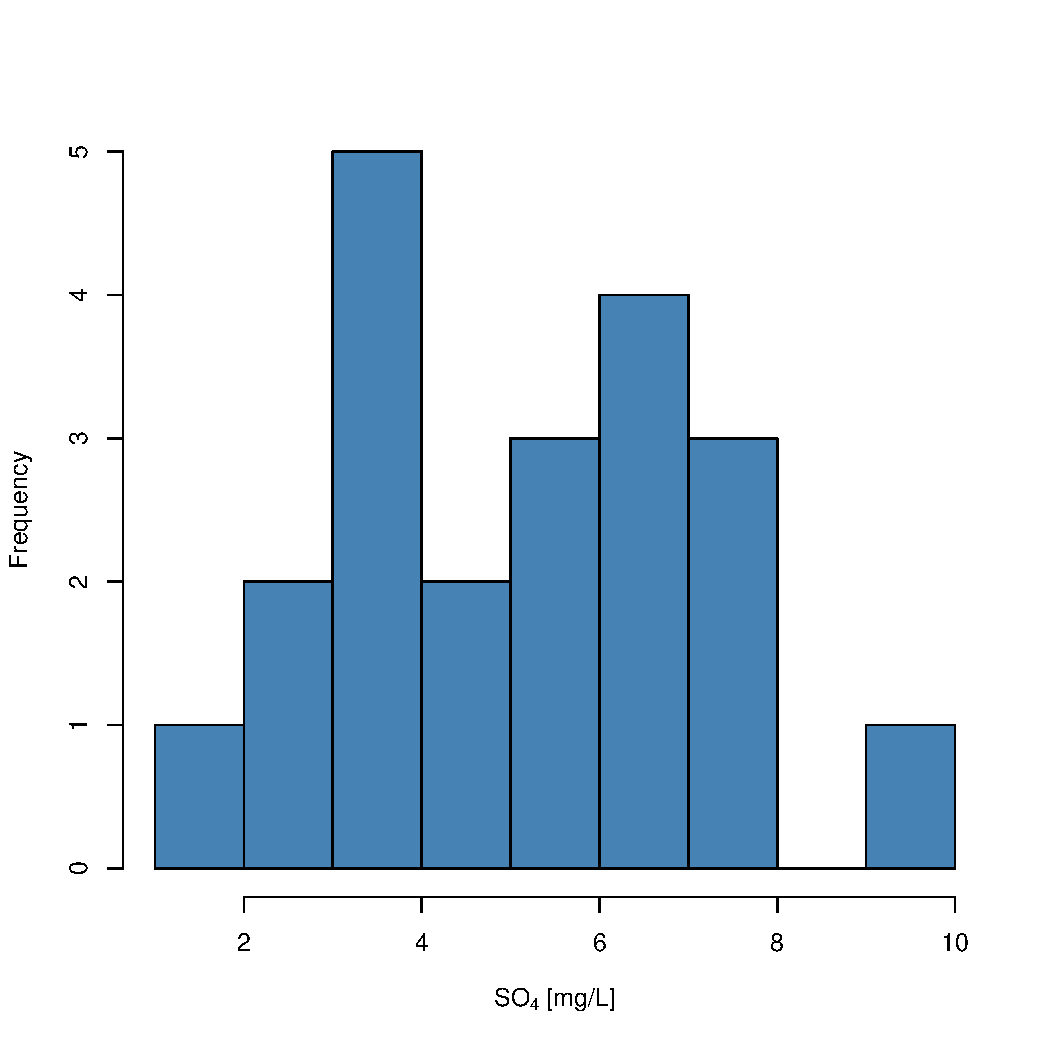
\includegraphics[width=\linewidth]{graphics/so4_hist} 

}



\end{knitrout}

\caption{A histogramm of the so4 data.}
\end{marginfigure}


\begin{knitrout}
\definecolor{shadecolor}{rgb}{0.969, 0.969, 0.969}\color{fgcolor}\begin{kframe}
\begin{alltt}
\hlstd{so4}
\end{alltt}
\begin{verbatim}
##  [1] 1.3 2.3 2.6 3.3 3.5 3.5 3.6 4.0 4.1 4.5 5.2 5.6
## [13] 5.7 6.1 6.2 6.5 6.9 7.1 7.7 7.9 9.9
\end{verbatim}
\begin{alltt}
\hlkwd{length}\hlstd{(so4)}
\end{alltt}
\begin{verbatim}
## [1] 21
\end{verbatim}
\begin{alltt}
\hlkwd{mean}\hlstd{(so4)}
\end{alltt}
\begin{verbatim}
## [1] 5.119
\end{verbatim}
\begin{alltt}
\hlkwd{sd}\hlstd{(so4)}
\end{alltt}
\begin{verbatim}
## [1] 2.137
\end{verbatim}
\end{kframe}
\end{knitrout}


So there are 21 measurements with a mean of 5.1 mg/L and a standard deviation 
of 2.1 mg/L. 

Suppose we have a detection limit of 2.5 mg/L and want to winsorize values below
LOD.

\newpage
To compute winsorized values we use \verb|winsor| function from the \verb|qetx| 
package.
This function takes a vector of values and a second argument specifying how 
many values should be winsorized (either by giving a LOD-value or the number of
values on each side) \sidenote{Take a look what computations are performed by 
looking at the source of this function - type the function name into the 
console}.

\begin{knitrout}
\definecolor{shadecolor}{rgb}{0.969, 0.969, 0.969}\color{fgcolor}\begin{kframe}
\begin{alltt}
\hlstd{so4_w} \hlkwb{<-} \hlkwd{winsor}\hlstd{(so4,} \hlkwc{lod} \hlstd{=} \hlnum{2.5}\hlstd{)}
\hlstd{so4_w}
\end{alltt}
\begin{verbatim}
##  [1] 2.6 2.6 2.6 3.3 3.5 3.5 3.6 4.0 4.1 4.5 5.2 5.6
## [13] 5.7 6.1 6.2 6.9 6.5 7.1 7.7 7.7 7.7
## attr(,"width")
## [1] 2
\end{verbatim}
\end{kframe}
\end{knitrout}


\begin{knitrout}
\definecolor{shadecolor}{rgb}{0.969, 0.969, 0.969}\color{fgcolor}\begin{kframe}
\begin{alltt}
\hlkwd{mean}\hlstd{(so4_w)}
\end{alltt}
\begin{verbatim}
## [1] 5.081
\end{verbatim}
\begin{alltt}
\hlkwd{sd}\hlstd{(so4_w)}
\end{alltt}
\begin{verbatim}
## [1] 1.792
\end{verbatim}
\begin{alltt}
\hlkwd{sd_winsor}\hlstd{(so4_w)}
\end{alltt}
\begin{verbatim}
## [1] 2.24
\end{verbatim}
\end{kframe}
\end{knitrout}




\section{Probability Plotting}




\chapter{Bioaccumulation}



\chapter{Tests for Detection of Chronic Lethal and Sublethal Stress}



\chapter{Lethal and Other Quantal Responses to Stress}
\section{Fitting dose-response models}



\chapter{Population and Metapopulation Effects}



\chapter{Community Effects}

\section{Species Richness}

\section{Analysing mesocosm data}

\section{Species Sensitivity Distributions}



%%
% The back matter contains appendices, bibliographies, indices, glossaries, etc.
\backmatter
\appendix

\chapter{R Session Info}
\begin{knitrout}
\definecolor{shadecolor}{rgb}{0.969, 0.969, 0.969}\color{fgcolor}\begin{kframe}
\begin{alltt}
\hlkwd{sessionInfo}\hlstd{()}
\end{alltt}
\begin{verbatim}
## R version 3.0.2 (2013-09-25)
## Platform: x86_64-pc-linux-gnu (64-bit)
## 
## locale:
##  [1] LC_CTYPE=en_US.UTF-8      
##  [2] LC_NUMERIC=C              
##  [3] LC_TIME=en_US.UTF-8       
##  [4] LC_COLLATE=en_US.UTF-8    
##  [5] LC_MONETARY=en_US.UTF-8   
##  [6] LC_MESSAGES=en_US.UTF-8   
##  [7] LC_PAPER=en_US.UTF-8      
##  [8] LC_NAME=C                 
##  [9] LC_ADDRESS=C              
## [10] LC_TELEPHONE=C            
## [11] LC_MEASUREMENT=en_US.UTF-8
## [12] LC_IDENTIFICATION=C       
## 
## attached base packages:
## [1] stats     graphics  grDevices utils     datasets 
## [6] methods   base     
## 
## other attached packages:
## [1] qetx_0.0.1 knitr_1.5 
## 
## loaded via a namespace (and not attached):
## [1] evaluate_0.5.1 formatR_0.9    highr_0.2.1   
## [4] stringr_0.6.2  tools_3.0.2
\end{verbatim}
\end{kframe}
\end{knitrout}



%\bibliography{sample-handout}
%\bibliographystyle{plainnat}
\printindex
\end{document}
